% Anonymous IEEE-style manuscript source for the six-page CINS limit.
% Confirm the final class against the official venue author kit before upload.
% Compile from docs/research_paper so that the relative figure path resolves:
%   latexmk -pdf interViv_cins2026_anonymous.tex
\documentclass[conference,a4paper]{IEEEtran}

\usepackage[utf8]{inputenc}
\usepackage[T1]{fontenc}
\usepackage{amsmath}
\usepackage{array}
\usepackage{booktabs}
\usepackage{graphicx}
\usepackage{microtype}
\usepackage{balance}
\usepackage{xurl}
\usepackage[hidelinks]{hyperref}

\title{interViv: Auditable Diagnostic Scoring for Technical Interview Practice}
\author{\IEEEauthorblockN{Anonymous Submission}}

\begin{document}

\maketitle

\begin{abstract}
Automated interview-practice systems can produce confident scores without
showing whether those scores generalize or which evidence supports their
feedback. We evaluate interViv's current deterministic short-answer scorer as
a diagnostic component rather than as a learner-readiness predictor. A
reproducible grader lab compares lexical similarity, pinned semantic similarity
plus an inspectable contradiction heuristic, and the current guarded pipeline
on the five-way SciEntsBank ($n=5{,}835$) and BEETLE ($n=1{,}258$) Core test
sets. interViv reaches macro-F1 0.246 and 0.161, below the semantic baseline's
0.335 and 0.277. It has the lowest off-topic false-positive rates (0.009 and
0.007) but also low off-topic recall (0.062 and 0.010), and it exposes no
contradiction signal (0/894 detected). Feedback statements have complete
structural evidence identifiers, but this does not establish citation
correctness. Ablations indicate domain-sensitive weighting: removing the
classifier aggregation term improves macro-F1 on both benchmarks. The findings
distinguish structural auditability from predictive performance and identify
calibration, relevance detection, contradiction handling, and human validation
as priorities for future work.
\end{abstract}

\begin{IEEEkeywords}
automated short-answer grading, diagnostic feedback, auditability, technical
interview practice, evidence tracing, benchmark evaluation
\end{IEEEkeywords}

\section{Introduction}

Practice systems for technical interviews combine two tasks that should be
evaluated separately: generating a useful question and judging the learner's
response. A fluent prompt generator can increase variety, but a scoring
component influences what the learner studies next. That component therefore
needs external benchmark evidence, explicit failure modes, and a trace from
each feedback statement to the scoring evidence that licensed it.

interViv is an interview-practice prototype whose current scorer combines
semantic, classifier, keyword, TF--IDF, knowledge-graph, entity, and
anti-gaming signals. Earlier descriptions emphasized the complete application
and small internal validation exercises. This paper narrows the contribution
to the diagnostic scorer. We exclude learner-readiness improvement, hiring
validity, and the non-blinded pilot from the empirical claim set.

Five-way SemEval classification is used as an external stress test rather than
as a claim that interViv was designed as a SemEval classifier. Its native
continuous score, guard state, and evidence outputs do not map perfectly to the
benchmark label space.

We ask two questions. \textbf{RQ1:} How reliably does interViv assess answer
quality and relevance relative to lexical and semantic baselines on external
short-answer benchmarks? \textbf{RQ2:} What performance--auditability
trade-offs emerge from interViv's guarded, evidence-traceable diagnostic
pipeline, particularly for relevance and contradiction handling?

The contributions are: (1) an auditability-first diagnostic architecture
separating generative question creation from traceable answer assessment; (2)
a reproducible external evaluation on SciEntsBank and BEETLE against lexical
and semantic baselines; and (3) a failure-mode and component-sensitivity
analysis exposing domain-sensitive calibration, conservative relevance
detection, and the absence of an explicit contradiction output.

\section{Related Work}

\subsection{Automated short-answer grading}

SciEntsBank and BEETLE were consolidated in SemEval-2013 Task~7 as five-way
student-response classification data~\cite{dzikovska2013}. Representation-based
grading progressed from lexical matching toward contextual encoders
\cite{haller2022}, including Sentence-BERT~\cite{reimers2019}. ASAG2024
highlights the continued difficulty of cross-question and cross-domain
generalization~\cite{meyer2024}. Recent response-level studies show that
aggregate metrics conceal difficulty-dependent collapse~\cite{cong2026} and
mid-range degradation~\cite{schleifer2026}. We therefore report accuracy and
macro-F1 together with targeted safety and evidence metrics rather than
treating one score as a complete evaluation.

\subsection{LLM grading and auditability}

LLM judges can scale rubric application, but reliability, bias, prompt
dependence, and interpretability remain open problems~\cite{haque2026,gu2026}.
A 2026 rubric-guided study found gains for a larger model but degradation for a
smaller model; it also observed rationales containing hallucinated rubric
elements~\cite{haque2026}. Cross-disciplinary ChatGPT grading similarly showed
consistency alongside leniency and compressed grade distributions
\cite{awashreh2026}. These findings motivate explicit evidence identifiers, but
identifiers alone cannot prove that a feedback claim is warranted.

\subsection{Adaptive interview systems}

AI interviewer research has begun to evaluate adaptive questioning at scale.
Panfilova et al. compare six models using 2,900 human annotations
\cite{panfilova2026}, while recent technical mock-interview work studies
readiness and confidence~\cite{gomez2025}. Those studies focus on interviewing
behavior or learner experience. Our narrower unit is the diagnostic judgment
attached to one answer and, synthetically, the resolution of one identified
competency gap.

\begin{table}[t]
\caption{Positioning relative to related research families.}
\label{tab:related-comparison}
\centering
\scriptsize
\setlength{\tabcolsep}{2.5pt}
\begin{tabular}{@{}lccccc@{}}
\toprule
Work & Ext. & Evid. & Det. & Adapt. & Failure \\
     & data & trace & score & context & analysis \\
\midrule
SemEval ASAG~\cite{dzikovska2013} & Yes & -- & Yes & -- & Yes \\
Rubric LLM~\cite{haque2026} & Yes & Partial & -- & -- & Yes \\
AI interviewer~\cite{panfilova2026} & -- & Partial & -- & Yes & Yes \\
\textbf{interViv} & Yes & Yes & Yes & Yes$^{*}$ & Yes \\
\bottomrule
\end{tabular}

\vspace{2pt}
\raggedright\scriptsize
$^{*}$Adaptivity exists in the platform but is not experimentally validated in
this paper. The structured LLM-judge comparison is deferred.
\end{table}

\section{Diagnostic Scoring and Evidence}

\subsection{Scoring boundary}

The research adapter calls the existing production scorer without changing
application logic. For an answer $a$ and reference $r$, the pipeline computes a
bounded semantic component, a saved logistic-regression component, keyword
coverage, and TF--IDF similarity. Knowledge-graph and entity bonuses are added,
penalties are subtracted, and any anti-gaming cap is applied last. The saved
classifier also consumes a semantic-derived feature; consequently, the
component ablations are sensitivity tests rather than causal isolation.

\begin{figure}[t]
  \centering
  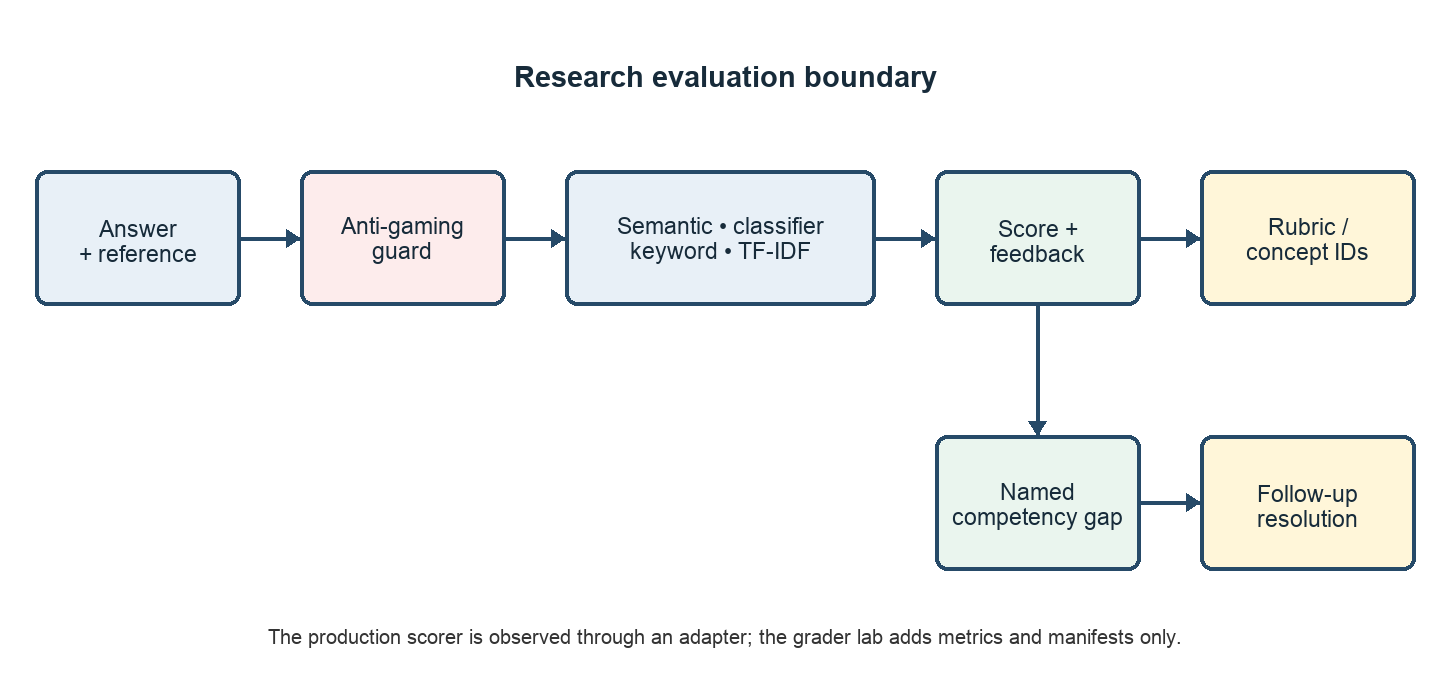
\includegraphics[width=\columnwidth]{figures/cins_fig01_diagnostic_pipeline.png}
  \caption{Diagnostic scoring, evidence, and follow-up boundary.}
  \label{fig:pipeline}
\end{figure}

The aggregate score is
\begin{equation}
\begin{split}
S = \min\bigl(C_g,\;&100(0.45s_{\mathrm{sem}}+0.25s_{\mathrm{clf}}\\
&+0.20s_{\mathrm{kw}}+0.10s_{\mathrm{tfidf}})\\
&+b_{\mathrm{KG}}+b_{\mathrm{NER}}-p\bigr).
\end{split}
\label{eq:score}
\end{equation}

\subsection{Diagnostic-output mapping}

Table~\ref{tab:mapping} distinguishes interViv's native capabilities from the
external SemEval label space. Five-way classification tests transfer behavior;
it does not imply that the production scorer was designed as a five-class
SemEval model.

\begin{table}[t]
\caption{Mapping from native diagnostics to external evaluation.}
\label{tab:mapping}
\centering
\scriptsize
\setlength{\tabcolsep}{3pt}
\begin{tabular}{@{}p{18mm}p{23mm}p{25mm}p{16mm}@{}}
\toprule
Capability & interViv output & SemEval mapping & Status \\
\midrule
Answer quality & Score and classifier & Correct or partial & Evaluated \\
Relevance & Guard signal & Irrelevant or non-domain & Evaluated \\
Contradiction & Not exposed & Contradictory & Gap found \\
Evidence provenance & Rubric/concept ID & No direct equivalent & Structural audit \\
\bottomrule
\end{tabular}
\end{table}

\subsection{Feedback evidence contract}

Every emitted feedback statement can list evidence IDs from an available set.
Rubric evidence uses \texttt{rubric.*} and concept evidence uses
\texttt{concept.*}. Evidence-citation completeness is the fraction of feedback
statements citing at least one valid rubric or concept ID. Unsupported-feedback
rate is computed separately from whether the citation is explicit. Both are
structural checks; human adjudication is required to establish substantive
support or pedagogical usefulness.

\subsection{Follow-up resolution}

A follow-up record names the exact trigger gap and whether the second answer
resolves it. Resolved-evidence rate is the accuracy of that exact-gap judgment.
SciEntsBank and BEETLE are single-turn data, so this metric is never reported as
benchmark validation; all corresponding rows carry
\texttt{pilot\_synthetic=true}.

\section{Evaluation}

\subsection{Data and labels}

We normalize the official SemEval five-way Core test partitions to a shared
JSONL schema: correct, partially correct/incomplete, contradictory, irrelevant,
and non-domain. SciEntsBank contributes 5,835 examples and BEETLE 1,258. Their
organizer package is CC BY-SA 3.0. An internal 17-example set covers off-topic,
vague, keyword-stuffed, contradictory, partial, clean-control, and four
follow-up cases. RiceChem is absent and recorded as
\texttt{pending\_access} rather than silently omitted.

\subsection{Baselines}

Lexical similarity uses content-token F1. The semantic baseline uses the pinned
\texttt{all-MiniLM-L6-v2} checkpoint plus an inspectable negation/antonym
heuristic; it is not a trained NLI model. The interViv baseline uses the current
scorer and guards. A structured LLM rubric-judge interface exists only as a
disabled configuration stub. It is marked \texttt{deferred}, made zero
API/network calls, and leaves this comparison \emph{incomplete}.

\subsection{Metrics and protocol}

We report five-way accuracy and macro-F1; off-topic recall and false-positive
rate; contradiction recall; unsupported-feedback rate; and evidence-citation
completeness. The synthetic follow-up pilot additionally reports exact-gap
resolution. All models run offline. The clean run records 7,110 applicable
interViv predictions, 7,110 semantic function calls, and zero lexical
fallbacks. No test-set tuning was performed after inspecting the results.

\subsection{Reproducibility manifest}

The primary run is \texttt{grader-lab-20260815T160016Z}; ablation is
\texttt{grader-lab-20260815T161227Z}; and contradiction analysis is
\texttt{grader-lab-20260815T161440Z}. All record commit
\texttt{8758ecfed517} (dirty research worktree), dataset versions and SHA-256
digests, Python/runtime versions, embedding revision \texttt{1110a243fdf4},
and classifier artifact \texttt{2897c8cc6283}. The frozen CSV/Markdown hashes
are listed in the supplemental experiment-freeze file.

\section{Results}

\subsection{Five-way grading}

On SciEntsBank, interViv improves accuracy over the lexical baseline (0.373
vs.\ 0.358) but is below the semantic baseline (0.399). Its macro-F1 (0.246) is
effectively the lexical result (0.245) and below semantic (0.335). On BEETLE,
interViv is worse in both accuracy (0.170) and macro-F1 (0.161) than lexical
(0.338, 0.274) and semantic (0.304, 0.277). RQ1 therefore has a negative answer:
the current aggregate does not generalize competitively across the two
benchmark domains.

\begin{table}[t]
\caption{Accuracy and macro-F1 (benchmark-validated).}
\label{tab:grading}
\centering
\small
\begin{tabular}{@{}lccc@{}}
\toprule
Dataset / metric & Lexical & Semantic & interViv \\
\midrule
SciEntsBank Accuracy & 0.358 & 0.399 & 0.373 \\
SciEntsBank Macro-F1 & 0.245 & 0.335 & 0.246 \\
BEETLE Accuracy      & 0.338 & 0.304 & 0.170 \\
BEETLE Macro-F1      & 0.274 & 0.277 & 0.161 \\
\bottomrule
\end{tabular}
\end{table}

\subsection{Safety and contradictions}

interViv produces the lowest off-topic false-positive rate on both datasets,
but this apparent safety is coupled to very low detection recall. SciEntsBank
recall/FPR is 0.062/0.009 versus lexical 0.407/0.141; BEETLE is 0.010/0.007
versus lexical 0.727/0.085. The semantic baseline offers a less extreme
trade-off. interViv detects 0/539 SciEntsBank and 0/355 BEETLE contradictions
because the current adapter exposes no contradiction output. The semantic
heuristic detects 170/539 and 148/355. Of its 576 misses, automatic rules
resolve only one as a factual reversal; 575 require human review.

\begin{table}[t]
\caption{Off-topic and contradiction metrics (benchmark-validated).}
\label{tab:safety}
\centering
\small
\begin{tabular}{@{}llccc@{}}
\toprule
Dataset & Baseline & OT recall & OT FPR & Contr. recall \\
\midrule
SciEntsBank & Lexical  & 0.407 & 0.141 & 0.000 \\
             & Semantic & 0.134 & 0.012 & 0.315 \\
             & interViv & 0.062 & 0.009 & 0.000 \\
\addlinespace
BEETLE      & Lexical  & 0.727 & 0.085 & 0.000 \\
             & Semantic & 0.626 & 0.021 & 0.417 \\
             & interViv & 0.010 & 0.007 & 0.000 \\
\bottomrule
\end{tabular}
\end{table}

\subsection{Auditability and follow-up pilot}

interViv feedback has 100\% evidence-citation completeness and zero
automatically unsupported claims in this run. However, the semantic research
baseline also reaches 100\% because its adapter emits evidence IDs, and the
deferred LLM judge prevents an opaque-judge comparison. The result supports
only a structural traceability claim. On four internal follow-up cases,
interViv and the semantic baseline each judge exact-gap resolution correctly in
4/4 cases; lexical obtains 3/4. This is synthetic-only pilot evidence, not a
learner-outcome result.

\subsection{Component sensitivity}

Removing the classifier final-score term improves macro-F1 from 0.246 to 0.251
on SciEntsBank and from 0.161 to 0.205 on BEETLE. Removing semantic evidence
lowers SciEntsBank macro-F1 to 0.231 but raises BEETLE to 0.179. Removing guards
raises SciEntsBank macro-F1 to 0.258 yet lowers BEETLE to 0.128 and eliminates
the explicit off-topic flag. The differences indicate domain-sensitive
calibration and a measurable guard trade-off, not one universally dominant
component.

\begin{table}[t]
\caption{Research-only macro-F1 ablations.}
\label{tab:ablation}
\centering
\small
\begin{tabular}{@{}lccc@{}}
\toprule
Configuration & SciEntsBank & BEETLE & Synthetic pilot$^{*}$ \\
\midrule
Full                 & 0.246 & 0.161 & 0.578 \\
$-$ semantic         & 0.231 & 0.179 & 0.267 \\
$-$ classifier term  & 0.251 & 0.205 & 0.567 \\
$-$ keyword term     & 0.246 & 0.159 & 0.523 \\
$-$ TF--IDF term     & 0.250 & 0.159 & 0.578 \\
$-$ guards           & 0.258 & 0.128 & 0.455 \\
\bottomrule
\end{tabular}
\vspace{0.25em}

\raggedright\footnotesize $^{*}$\texttt{pilot\_synthetic=true}; not benchmark evidence.
\end{table}

\section{Discussion and Limitations}

The strongest current result is diagnostic rather than promotional. Semantic
execution is verified, so the poor BEETLE result cannot be explained by a
silent lexical fallback. The combination of low false positives and very low
recall indicates that the guard is conservative. The classifier-term ablation
and opposite semantic effect across domains identify calibration as a priority
for future work. Contradiction detection is a missing capability at the
scorer-output boundary, not merely a threshold problem.

Predictive performance and auditability are independent properties. A system
may be accurate but opaque, traceable but poorly calibrated, both, or neither.
interViv currently demonstrates structural traceability while requiring better
calibration and richer diagnostic signals. This separation is important because
the presence of an evidence ID cannot compensate for an incorrect prediction,
and a strong aggregate score cannot by itself make feedback inspectable.

The evaluation has several limits. First, benchmark labels do not cleanly
isolate low effort, so the off-topic result cannot be generalized to every
low-effort answer. Second, the contradiction taxonomy is almost entirely
unresolved without human review. Third, citation completeness checks the
presence of valid IDs, not the truth, sufficiency, or pedagogical quality of a
statement. Fourth, the four follow-ups are constructed examples. Fifth, the
structured LLM judge is deferred and RiceChem is pending, so the comparison is
explicitly incomplete.

No result here establishes improved readiness, retention, fairness across
learner groups, or hiring validity. Those claims require a consented
longitudinal study with blinded human adjudication. The earlier non-blinded
pilot is excluded from the main evidence. Future research should add an
independently adjudicated contradiction set, calibrate on development data
without touching the test partitions, implement the structured-judge
comparison under an approved cost/privacy policy, and collect real follow-up
conversations.

\section{Conclusion}

A reproducible evaluation of interViv's current diagnostic scorer finds
complete structural evidence tracing and low off-topic false positives, but
weak off-topic recall, no contradiction output, and substantial cross-domain
calibration failure. The semantic baseline outperforms the current aggregate on
macro-F1 in both external benchmarks. Treating these as first-class negative
results converts an application description into a falsifiable research
artifact. Stronger claims about LLM comparison, follow-up resolution, or
learner readiness remain deferred until the missing baselines and human studies
exist.

\balance
\begin{thebibliography}{11}
\small

\bibitem{dzikovska2013}
M. Dzikovska et al., ``SemEval-2013 Task 7: The Joint Student Response Analysis
and 8th Recognizing Textual Entailment Challenge,'' in \emph{Proc. SemEval},
2013, pp. 263--274.

\bibitem{haller2022}
S. Haller, A. Aldea, C. Seifert, and N. Strisciuglio, ``Survey on automated
short answer grading with deep learning: From word embeddings to
transformers,'' arXiv:2204.03503, 2022.

\bibitem{reimers2019}
N. Reimers and I. Gurevych, ``Sentence-BERT: Sentence embeddings using Siamese
BERT-networks,'' in \emph{Proc. EMNLP-IJCNLP}, 2019, pp. 3982--3992.

\bibitem{meyer2024}
G. Meyer, P. Breuer, and J. F{\"u}rst, ``ASAG2024: A combined benchmark for
short answer grading,'' in \emph{Proc. SIGCSE Virtual}, 2024,
doi:10.1145/3649409.3691083.

\bibitem{cong2026}
L. Cong, S. Hahn, S. Gombert, L. Camus, H. Drachsler, and U. Kroehne,
``Estimating LLM grading ability and response difficulty in automatic short
answer grading via item response theory,'' in \emph{Proc. BEA}, 2026,
pp. 259--271, doi:10.18653/v1/2026.bea-1.19.

\bibitem{schleifer2026}
A. Gurin Schleifer, M. Ariely, B. Beigman Klebanov, A. Salman, and
G. Alexandron, ``Quality-conditioned agreement in automated short answer
scoring,'' in \emph{Proc. BEA}, 2026, pp. 432--442,
doi:10.18653/v1/2026.bea-1.29.

\bibitem{haque2026}
S. Haque, D. Hettiachchi, and D. Beck, ``Rubric-guided prompting for automatic
assessment scoring,'' in \emph{Proc. L@S}, 2026, pp. 428--432,
doi:10.1145/3774398.3811581.

\bibitem{gu2026}
J. Gu et al., ``A survey on LLM-as-a-judge,'' \emph{The Innovation}, vol. 7,
no. 6, Art. 101253, 2026, doi:10.1016/j.xinn.2025.101253.

\bibitem{awashreh2026}
R. Awashreh, H. Al Ghunaimi, and S. AlGhenaimi, ``Reliable but not rigorous:
Evaluating ChatGPT's reliability, validity, and bias in automated academic
grading,'' \emph{Social Sciences \& Humanities Open}, Art. 102788, 2026,
doi:10.1016/j.ssaho.2026.102788.

\bibitem{panfilova2026}
A. Panfilova et al., ``The AI interviewer: Multi-faceted evaluation of adaptive
questioning by large language models,'' \emph{Scientific Reports}, vol. 16,
Art. 20257, 2026, doi:10.1038/s41598-026-46517-7.

\bibitem{gomez2025}
N. Gomez, S. S. Batham, M. Volonte, and T. D. Do, ``Virtual interviewers, real
results: Exploring AI-driven mock technical interviews on student readiness
and confidence,'' arXiv:2506.16542, 2025.

\end{thebibliography}

\end{document}
